% File: solutions/ex23.tex

\begin{soluzione}{23}
    \begin{enumerate}
        \item \textbf{Analisi e Grafico dello Spettro Originale $X(f)$}
        
        Lo spettro $X(f)$ è la convoluzione di due funzioni rettangolari:
        \begin{itemize}
            \item $G(f) = \text{rect}\left(\frac{f}{8}\right)$: un rettangolo di altezza 1 e larghezza 8, esteso da -4 Hz a 4 Hz. La sua banda è $B_g = 4$ Hz.
            \item $H(f) = \text{rect}\left(\frac{f}{4}\right)$: un rettangolo di altezza 1 e larghezza 4, esteso da -2 Hz a 2 Hz. La sua banda è $B_h = 2$ Hz.
        \end{itemize}
        
        La convoluzione di due rettangoli centrati nell'origine produce una funzione a forma di \textbf{trapezio}. Le sue caratteristiche sono:
        \begin{itemize}
            \item \textbf{Banda:} La banda del risultato è la somma delle bande individuali.
            \[
                B = B_g + B_h = 4 \text{ Hz} + 2 \text{ Hz} = \mathbf{6 \text{ Hz}}
            \]
            Lo spettro è quindi non nullo nell'intervallo $[-6, 6]$ Hz.
            
            \item \textbf{Ampiezza Massima:} L'ampiezza massima (l'altezza del trapezio) è data dall'area del rettangolo più piccolo.
            \[
                \text{Area di } H(f) = \text{altezza} \times \text{larghezza} = 1 \times 4 = 4
            \]
            Quindi, l'ampiezza massima di $X(f)$ è \textbf{4}.
            
            \item \textbf{Base Superiore del Trapezio:} La larghezza della parte piatta superiore è data dalla differenza delle larghezze dei rettangoli: $|8 - 4| = 4$ Hz. La parte piatta si estende quindi da $-2$ Hz a $2$ Hz.
        \end{itemize}
        
        Il grafico di $X(f)$ è:
        \begin{center}
        \begin{tikzpicture}
            \begin{axis}[
                axis lines=middle, xlabel=$f$ (Hz), ylabel=$X(f)$,
                xmin=-7, xmax=7, ymin=0, ymax=5,
                xtick={-6, -2, 0, 2, 6}, ytick={4},
            ]
            \addplot[blue, thick] coordinates {(-6,0) (-2,4) (2,4) (6,0) -- cycle};
            \end{axis}
        \end{tikzpicture}
        \end{center}
        
        \item \textbf{Grafico dello Spettro Campionato $\tilde{X}(f)$}
        
        Verifichiamo la condizione di Nyquist: $f_s \ge 2B \implies 10 \ge 2 \cdot 6 \implies 10 \ge 12$. La condizione è \textbf{violata}, quindi si verifica aliasing.
        
        Lo spettro campionato è una ripetizione di $X(f)$ con periodo $f_s = 10$ Hz, e l'ampiezza è scalata di $f_s=10$. Il picco del trapezio diventa $4 \cdot 10 = 40$.
        
        \begin{itemize}
            \item La replica centrale ($k=0$) si estende da $-6$ a $6$ Hz.
            \item La replica di destra ($k=1$), centrata a $10$ Hz, si estende da $10-6=4$ Hz a $10+6=16$ Hz.
            \item La replica di sinistra ($k=-1$), centrata a $-10$ Hz, si estende da $-16$ Hz a $-4$ Hz.
        \end{itemize}
        La sovrapposizione avviene dove le code si incontrano, cioè negli intervalli $[-6, -4]$ e $[4, 6]$.
        
        \begin{center}
        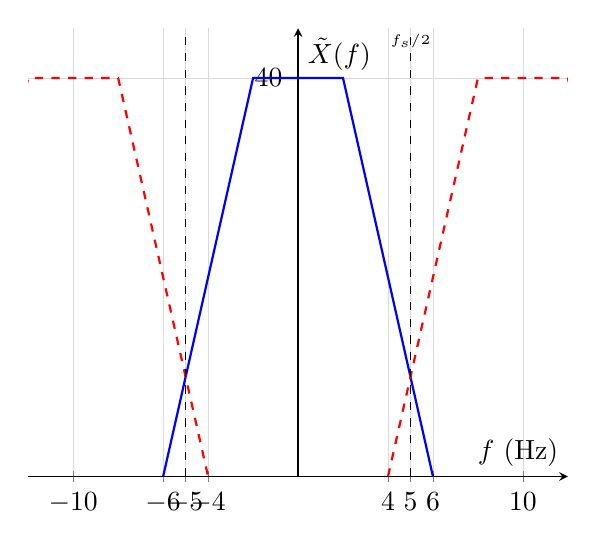
\begin{tikzpicture}
            \begin{axis}[
                axis lines=middle, xlabel=$f$ (Hz), ylabel=$\tilde{X}(f)$,
                xmin=-12, xmax=12, ymin=0, ymax=45,
                xtick={-10, -6, -5, -4, 0, 4, 5, 6, 10}, ytick={40},
                grid=both, grid style={line width=.1pt, draw=gray!30},
            ]
            % Replica centrale (k=0)
            \addplot[blue, thick] coordinates {(-6,0) (-2,40) (2,40) (6,0)};
            % Replica destra (k=1)
            \addplot[red, thick, dashed] coordinates {(4,0) (8,40) (12,40) (16,0)};
            % Replica sinistra (k=-1)
            \addplot[red, thick, dashed] coordinates {(-16,0) (-12,40) (-8,40) (-4,0)};
            % Banda di Nyquist
            \draw[dashed, black] (axis cs:-5,0) -- (axis cs:-5,45);
            \draw[dashed, black] (axis cs:5,0) -- (axis cs:5,45);
            \node[above,font=\tiny] at (axis cs:5, 42) {$f_s/2$};
            \end{axis}
        \end{tikzpicture}
        \end{center}
        
        \item \textbf{Grafico dello Spettro Normalizzato $\tilde{X}(\nu)$}
        
        Per ottenere questo grafico, riscaliamo l'asse delle frequenze del grafico precedente per $f_s=10$. La relazione è $\nu = f/10$.
        \begin{itemize}
            \item $f=\pm 4 \implies \nu=\pm 0.4$
            \item $f=\pm 6 \implies \nu=\pm 0.6$
            \item $f=\pm 10 \implies \nu=\pm 1$
        \end{itemize}
        Il periodo dello spettro normalizzato è 1.
        
        \begin{center}
        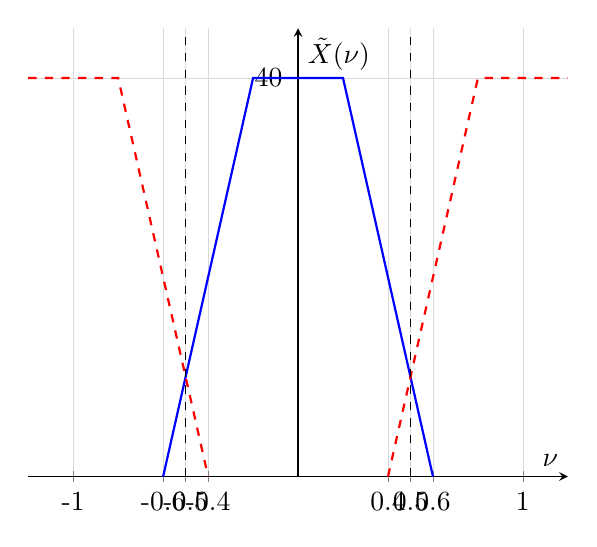
\begin{tikzpicture}
            \begin{axis}[
                axis lines=middle, xlabel=$\nu$, ylabel=$\tilde{X}(\nu)$,
                xmin=-1.2, xmax=1.2, ymin=0, ymax=45,
                xtick={-1, -0.6, -0.5, -0.4, 0, 0.4, 0.5, 0.6, 1},
                xticklabels={-1, -0.6, -0.5, -0.4, 0, 0.4, 0.5, 0.6, 1},
                ytick={40},
                grid=both, grid style={line width=.1pt, draw=gray!30},
            ]
            % Replica centrale (k=0)
            \addplot[blue, thick] coordinates {(-0.6,0) (-0.2,40) (0.2,40) (0.6,0)};
            % Replica destra (k=1)
            \addplot[red, thick, dashed] coordinates {(0.4,0) (0.8,40) (1.2,40)};
            % Replica sinistra (k=-1)
            \addplot[red, thick, dashed] coordinates {(-1.2,40) (-0.8,40) (-0.4,0)};
            % Banda di Nyquist
            \draw[dashed, black] (axis cs:-0.5,0) -- (axis cs:-0.5,45);
            \draw[dashed, black] (axis cs:0.5,0) -- (axis cs:0.5,45);
            \end{axis}
        \end{tikzpicture}
        \end{center}
        
    \end{enumerate}
\end{soluzione}